\documentclass[xetex,mathserif,serif]{beamer}
\usetheme{Frankfurt}
%\usecolortheme{beaver}
%\usecolortheme{dolphin}
\usecolortheme{beaver}
% \usepackage{nips10submit_e,times}
% setfont command is only available after usepackage{fontspec}
% \usepackage{ifxetex}
% \ifxetex
\usepackage{fontspec}
\usepackage{xltxtra}
% \usepackage[sc]{mathpazo}
% \usepackage[BoldFont,CJKnumbb] {xeCJK}
% \defaultfontfeatures{Ligatures={Common}, Mapping={tex-text}}
\setmainfont{Minion Pro}
%\setbeamerfont{title}{family=\rm\addfontfeatures{Scale=1.18, Numbers={Lining, Proportional}}}
% \setsansfont{Minion Pro}
% \setmonofont[Scale=0.8]{Monaco}
%   % \setCJKmainfont{Adobe Song Std}
%   % \XeTeXlinebreaklocale "zh"
%   % \XeTeXlinebreakskip = 0pt plus 1pt
% \else

%\usepackage[sc]{mathpazo}
%\usepackage[T1]{fontenc}
% \fi

% converts LaTeX specials (``quotes'' --- dashes etc.) to unicode

% \setromanfont{Liberation Serif} % Roman font is Serif font, \setromanfont has been
% replaced by \setmainfont
% \RequirePackage{mathptmx}
% \setromanfont{FreeSerif}

% can't find free version of Electra LH fonts
% \setromanfont [Mapping=tex-text,Ligatures={Common},BoldFont={ElectraLH-Bold},ItalicFont={ElectraLH-CursiveOsF},BoldItalicFont={ElectraLH-BoldCursiveOsF},SmallCapsFont={ElectraLH-RegularSC}]{ElectraLH-RegularOsF}
% \setsansfont[Mapping=tex-text,BoldFont={Delicious-Bold},ItalicFont={Delicious-Italic},SmallCapsFont={Delicious-SmallCaps}] {Delicious-Roman}


% \usepackage{cmbright}
% \renewcommand\sfdefault{phv}% use helvetica for sans serif
% \renewcommand\familydefault{\sfdefault}% use sans serif by default
% \usepackage[dvipsnames,usenames]{xcolor}
% \usepackage[opticals,medfamily,minionint,footnotefigures]{MinionPro}
\AtBeginSection[] {
  \begin{frame}[plain]
    \frametitle{Overview}
    \tableofcontents[currentsection]
  \end{frame}
  \addtocounter{framenumber}{-1}
}
\graphicspath{{./figures/}}
\usepackage[lotdepth, lofdepth]{subfig}
\usepackage{ucs}
%\usepackage[utf8]{inputenc}

% \usepackage[final,expansion=true,protrusion=true,spacing=true,kerning=true]{microtype}
\usepackage{amsmath, epsfig}
\usepackage{amsfonts}
% \usepackage{amssymb}
\usepackage{algorithm}
\usepackage{algorithmic}
% \usepackage{easybmat}
\usepackage{footmisc}
\usepackage{bm}
% \usepackage{fullpage}
\graphicspath{{./figures/}}
\DeclareGraphicsExtensions{.pdf,.png,.jpg}
\renewcommand\algorithmiccomment[1]{// \textit{#1}}
\newcommand\independent{\protect\mathpalette{\protect\independenT}{\perp}}
\def\independenT#1#2{\mathrel{\rlap{$#1#2$}\mkern2mu{#1#2}}}
%

\title{Bayesian Hierarchical Models with Applications in Meta-analysis and
  Large-scale Survey} \author{Wei Wang \\ Oral Examination for the degree of \\
  Master of Philosophy in the subject of \\ Statistics} 

\date{Dec 2\textsuperscript{th}, 2013}

\begin{document}

\frame{\titlepage}

% \section[Outline]{}
% \frame{\tableofcontents}
%
% \section{Introduction}
% \subsection{Overview of Topics}
%
% \section{Bayesian Analysis}
% \subsection{Single Parameter Model}

\begin{frame}
  \frametitle{Bayesian Hierarchical Models}
  \begin{itemize}
  \item The overarching theme of the following projects is the use of Bayesian
    hierarchical models (Multilevel models, or in Frequentist parlance, Empirical
    Bayes models, Random-effects/Mixed-effects models).
    \vskip 12pt
  \item In a nutshell, Bayesian hierarchical models regularize the fit of data
    with group structure through "partial pooling" across groups and provide more
    stable estimates.
  \end{itemize}
\end{frame}
\begin{frame}
  \frametitle{Overview}
  \tableofcontents[hideallsubsections]
\end{frame}
\section[Meta-analysis]{Hierarchical Non-parametric Models for Individual-level
  Meta-analysis}
\subsection{A Causal Framework for Meta-analysis}
\begin{frame}
  \frametitle{Meta-analysis}
  \begin{itemize}
  \item Meta-analyses synthesize evidence from multiple studies.

  \item Traditionally, meta-analysis researchers go through thorough literature
    reviews and data extractions.  

  \item Increasingly, researchers begin to have access to original data from a
    suite of studies and individual-level meta-analysis becomes feasible.
  \end{itemize}
\end{frame}

\begin{frame}
  \frametitle{Potential Outcomes and Causal Inference}
  \begin{itemize}
  \item Potential outcome framework is the standard tool for causal inference
    (Neyman, 1923; Rubin 1977). 
  \item The key insight is to consider the individual's responses subject to all
    possible treatment assignments $\vec Y=(Y(1), Y(2), \ldots, Y(L))$.
  \item Consider the case of binary treatment, we define causal estimands such as
    unit causal effect $Y_i(1)-Y_i(0)$, population average causal effect
    $E(Y_i(1)-Y_i(0))$ and conditional average causal effect $E(Y_i(1)-Y_i(0)|X)$.
    \pause
  \item However, meta-analysis researchers rarely take on the potential outcome
    framework even though most of meta-analysis target at causal conclusions.
  \end{itemize}
\end{frame}

\begin{frame}
  \frametitle{Heterogeneity in Meta-analysis}
  \begin{itemize}
  \item There are several statistical issues in meta-analysis, including
    publication bias, choices of effect parameters and study qualities.
    \pause
  \item Heterogeneity of effects across studies attracts most methodological
    research.  \pause
  \item Random-effects model (DerSimonion and Laird 1986) is the most popular
    choice, which gives that effect sizes $\hat\theta_i$ from different studies a
    prior distribution.
    \[\hat\theta_i=\theta_i+\varepsilon_i, \theta_i\sim \Psi(\cdot)\]
  \end{itemize}
\end{frame}

\begin{frame}
  \frametitle{An Extended Potential Outcome for Meta-analysis}
  \begin{itemize}
  \item Sobel et al. (2013) lays out an extended potential outcome framework for
    meta-analysis.
  \item The extended potential outcome for meta-analysis is to consider all
    possible outcomes that individual $i$ can experience under every combination
    of study membership $s\in\{1,\ldots,G\}$ and treatment assignment
    $z\in\{1,\ldots,L\}$,
    \begin{equation*}
      \label{eq:fpo}
      \bm \vec Y_i=
      \begin{pmatrix}
        Y_i(1,1) & Y_i(1,2) & \cdots & Y_i(1,L)\\
        Y_i(2,1) & Y_i(2,2) & \cdots & Y_i(2,L)\\
        \vdots & \vdots & \ddots & \vdots\\
        Y_i(G,1) & Y_i(G,2) & \cdots & Y_i(G,L)
      \end{pmatrix}.
    \end{equation*}
  \end{itemize}
\end{frame}

\begin{frame}
  \frametitle{Consistency Assumptions}
  \begin{itemize}
  \item[A1] Extended stable unit treatment value assumption: $\vec Y_i(\vec
    s,\vec z)=Y_i(s_i, z_i)$ for all possible $s$ and $z$.
  \item[A2] Sampling assumption: \[Y_i|s,z,x\stackrel{i.i.d.}{\sim}F(y|s,z,x).\]
  \item[A3] Response consistency:
    \[p(y(s,z)|S=s^{\prime\prime},Z=z, X=x)=p(y(s^\prime,z)|S=s^{\prime\prime},
    Z=z,X=x),\forall s,s^\prime,s^{\prime\prime},z, x.\]
  \end{itemize}
\end{frame}

\begin{frame}
  \frametitle{Selection Assumptions}
  \begin{itemize}
  \item[A6] Strongly ignorable treatment assignment:\\
     \[\{Y(s,z):s = 1,...,G, z = 1,...,L\} \independent Z\mid S = s, X_1 =
     x_1\] and
     \[0<P(Z=z\mid S=s, X_1=x_1)<1, \text{ for seen combinations of } s \text{
       and }z.\]
   \item[A7] Ignorable study selection: \\
     \[\{Y(s,z): s = 1,...,G, z = 1,...,L\} \independent S \mid X_2\]
  \end{itemize}
\end{frame}


\begin{frame}
  \frametitle{Two Sources of Heterogeneity}
  \begin{itemize}
  \item Assumption (A1) (A2) and (A6) have standard counterparts in causal
    inference of a single study.  
    \pause
  \item Extended potential outcome framework provides insights into the possible
    sources of heterogeneity that could be introduced into meta-analysis.
    \pause
  \item First, the violation of the response consistency assumption (A3).
  \item Second, the violation of the no study selection assumption (A7).
  \end{itemize}
\end{frame}

\begin{frame}
  \frametitle{Two Sources of Heterogeneity Cont'd}
  \begin{itemize}
  \item These two sources are inherently different and it might not be meaningful
    to use a model that blends these two.
  \item Traditional methods for meta-analysis make no distinction between these
    two sources.
    \pause
  \item As common in causal inference, assessing the validity of a particularly
    assumption is very important for practical modeling choice and analysis.
  \end{itemize}
\end{frame}

\begin{frame}
  \frametitle{Two Sources of Heterogeneity Cont'd}
  \begin{itemize}
  \item If (A7) is reasonable and (A3) is unlikely to hold, then the
    heterogeneity is the result of treatment effect variations across studies. In this
    case, a random-effects model might be warranted.
    \pause
  \item If (A3) is reasonable and (A7) is unlikely to hold, then the
    heterogeneity is the result of differential selection into studies. In this
    case, random-effects models are questionable.
  \end{itemize}
\end{frame}

\subsection{An Application to Vioxx Trials}
\begin{frame}
  \frametitle{Vioxx Example}
  \begin{itemize}
  \item In Sobel et al. (2013), an illustrative example of Vioxx is used to
    demonstrate the use of the potential outcome framework.
  \item Vioxx is a COX-2 selective, non-steroidal anti-inflammatory drug (NSAID)
    that was approved by the FDA for the relief of signs and symptoms of
    osteoarthritis, the management of acute pain in adults, and the treatment of
    menstrual symptoms.
  \item It was withdrawn from the market several years later as clinical trials
    began to reveal severe negative impact on cardiovascular system.
  \end{itemize}
\end{frame}

\begin{frame}
  \frametitle{Analysis of the Vioxx Example}
  \begin{itemize}
  \item We conducted a meta-analysis of 29 Vioxx trials finished before the
    withdrawal of Vioxx. In particular, we separate different dosages in our
    analysis.  \pause
  \item In this context, we deem assumption (A3), the response consistency
    assumption, as reasonable; this means that any heterogeneity will be the
    results of differential selection into studies.  
    \pause
  \item This leads to the use of study indicators and fixed-effects models rather
    than random-effects models. The meta-analysis confirms the negative impact of
    Vioxx on cardiovascular system, and differentiation of dosage leads to the
    finding of dosage-response relation that was ignored in previous Vioxx
    studies.
  \end{itemize}
\end{frame}
\subsection{A Bayesian Approach}
\begin{frame}
  \frametitle{A Bayesian Approach}
  \begin{itemize}
  \item There are situations where the treatment response consistency might not
    hold, e.g., in an education intervention program, an intervention is carried
    out by different teachers. In this case, a random-effects model might be
    warranted.
    \pause
  \item In this case, we would like to build a formal Hierarchical Bayesian
    framework.
  \end{itemize}
\end{frame}

\begin{frame}
  \frametitle{Hierarchical Bayesian Framework}
  \begin{itemize}
  \item The group structure of the extended potential outcome naturally lends
    itself to Hierarchical Bayesian Framework. For one individual under one
    treatment assignment, a total number of $G$ outcomes could have been
    experienced. In machine learning literature, this is known as multi-task
    learning problem.
    \pause
  \item The key insight is that parietal pooling across studies should help us
    improve our estimates.
    \pause
  \item A major problem is that the proportion of missingness is very high.
  \end{itemize}
\end{frame}

\subsection{Non-parametric Models for Causal Inference}
\begin{frame}
  \frametitle{Non-parametric Methods in Causal Inference}
  \begin{itemize}
  \item Causal inference in observational studies often involves fitting two
    models: a model for treatment assignment given variables pertinent to the
    selection process and a model for the potential outcomes given treatment and
    confounding variables. Rubin (2005) refers to the former as the model for
    selection and the latter as the model for science.
    \pause
  \item Mostly, simple parametric models, e.g., linear least square regression,
    are used to fit the selection model and potential outcome
    model. Considerations for missepcification leads to the popular doubly robust
    method (Scharfstein, Rotnitzky and Robins 1999).  
    \pause
  \item However, there have been a growing interest in developing flexible
    non-parametric models for the potential outcomes. Hill (2011) uses Bayesian
    Additive Regression Tree (BART) to model the potential outcomes without fitting the
    selection models.
  \end{itemize}
\end{frame}

\begin{frame}
  \frametitle{Gaussian Processes}
  \begin{itemize}
  \item Gaussian Process is another highly-flexible and also computationally
    attractive non-parametric model.
  \item A random function $f$ follows a Gaussian Process if its arbitrary finite
    distribution follows a multivariate Gaussian distribution, i.e.,
    $f(x_1,x_2,\ldots,x_n)\sim N(\mu(\vec x), K(\vec x, \vec x)), \forall n$,
    where $\kappa$ is the kernel that describes the underlying Gaussian process
    and $K(\vec x, \vec x)=(\kappa(x_i, x_j)))_{n\times n}$ is the Gram matrix.
  \item Gaussian Process is also used to model the mean function of a regression
    $y=f(x)+\varepsilon$, while the observational noise $\varepsilon$ is often
    given a normal distribution $N(0, \sigma^2)$.
  \end{itemize}
\end{frame}

\begin{frame}
  \frametitle{Incorporating Group Structure into Gaussian Processes}
  \begin{itemize}
  \item In the context of meta-analysis, each study has its own mean function
    $f_s$, which is a function of the treatment $z$ and confounders $x$, that
    follows a Gaussian process with kernel $\kappa_s$.
    \pause
  \item Bonilla (2008) proposes to decompose $\kappa_s=\tilde\kappa\cdot\check\kappa$, in
    which $\tilde\kappa$ describes "inter-task similarities" based on task-level
    characteristics, and $\check\kappa$ describes the similarity resulting from
    individual characteristics.
  \end{itemize}
\end{frame}

\begin{frame}
  \frametitle{Hierarchical Gaussian Processes}
  \begin{itemize}
  \item Another approach is to give the $\kappa_s$'s a prior distribution. This
    is discussed in Yu et al. (2004) and Schwaighofter et al. (2005).
  \item Restricting the infinite dimensional kernel function $\kappa_s$ on the
    $N$ individual observed in the data as the Gram matrix $K^s$, we can assign a
    standard Wishart prior with a base kernel $\kappa_0$, whose Gram matrix is $K_o$
    \[Q(K_s)\sim \text{InvW}(\tau, K_0),  s=1,\ldots,G\]
  \end{itemize}
\end{frame}

\begin{frame}
  \frametitle{Future work}
  \begin{itemize}
  \item Develop Hierarchical Gaussian Process models, specifically with the high
    "missingness" of the potential outcome framework in mind.
    \pause
    \vskip 12pt
  \item Gaussian process is natural for continuous responses, while there are
    other rapid development in Bayesian nonparametric models for data types such
    as count data and time-to-event data.
  \end{itemize}
\end{frame}

\begin{frame}
  \frametitle{References}
  \begin{itemize}
  \item Sobel, Michael and Madigan, David and Wang, Wei, 2013. Meta-Analysis: a
    causal framework, with application to randomized studies of Vioxx. Technical
    Report
  \item Rubin, Donald, 2005. Causal Inference Using Potential Outcomes. JASA.
  \item Schwaighofer, Anton and Tresp, Volker and Yu, Kai, 2004. Learning
    gaussian process kernels via hierarchical bayes. NIPS.
  \item Yu, Kai and Tresp, Volker and Schwaighofer, Anton, 2005. Learning Gaussian
    processes from multiple tasks. ICML.
  \item Bonilla, Edwin and Chai, Kian Ming and Williams, Christopher,
    2008. Multi-task Gaussian process prediction. ICML.
  \item Hill, Jennifer, 2011. Bayesian Nonparametric Modeling for Causal
    Inference. JCGS.
  \end{itemize}
  
\end{frame}
\section[Highly Nonrepresentative Polls]{Accurate Prediction Using Highly Nonrepresentative Online Survey Data via MRP
  Correction}
\subsection{Introduction}
\begin{frame}
  \frametitle{Introduction}
  \begin{itemize}
  \item National Survey data is another example that Bayesian Hierarchical Models
    could be a vital tool.
  \item Typically, national survey data is cross-tabulated by
    categorical geographical-demographic variables. (It is a common practice to
    discretize continuous variables such as age and income.) This creates a complex
    group structure. 
    \pause
  \item Multilevel Regression and Poststratification (MRP) takes advantage of
    this structure and is popular in small-area estimation at state level and
    sub-state level (Park et al., 2004; Lax and Phillips, 2009; Ghitza and
    Gelman, 2013 ).
  \item We apply MRP technique to a highly-biased online survey data set to
    construct accurate state-level prediction for 2012 Presidential Election.
  \end{itemize}
\end{frame}
\subsection{MRP}
\begin{frame}
  \frametitle{Multilevel Regression and Poststratification}
  \begin{itemize}
  \item The core idea of MRP is to partition the data set into small cells, use
    the sample to estimate the proportion in each cells via multilevel
    regression, and then aggregate the cell-level proportion to the
    population-level proportion by reweighting each cell according to the
    population information.
    \[\hat{y}^{\text{PS}}=\frac{\sum_{j=1}^JN_j\hat{y}_j}{\sum_{j=1}^JN_j}\]
  \item However, there is a trade-off between how fine we want to partition the
    data and the sample sizes within the small cells. The multilevel regression
    facilitates "borrowing strength" across demographically/geographically
    similar cells, and thus producing more stable cell-level estimates.
  \end{itemize}
\end{frame}
\subsection{Xbox Data}
\begin{frame}
  \frametitle{Description of the Xbox Data Set}
  \begin{itemize}
  \item An opt-in poll was placed on Xbox gaming platform daily in the period
    leading up to the 2012 US Presidential Election. 
  \item Users' daily voting intent as well as their demographic information was
    collected.
  \item In total, 750,148 interviews were conducted with 345,858 unique
    respondents—over 30,000 of whom completed five or more polls—making this one
    of the largest ever election panel studies.
  \end{itemize}
\end{frame}

\begin{frame}
  \frametitle{But Highly Nonrepresentative...}
  \begin{itemize}
  \item However, the survey is highly biased in gender and age. 93\% respondents
    are male and 65\% are 18-to-29-year-olds. The raw result is drawn below
    \begin{figure}[htbp]
      \centering
      \includegraphics[width=.7\textwidth]{"raw_response"}
      \caption{Raw results of the Xbox data.}
      \label{fig:raw}
    \end{figure}
  \end{itemize}
\end{frame}

\begin{frame}
  \frametitle{Is nonrepresentative survey salvageable?}
  \begin{itemize}
  \item The nonrepresentative nature of the Xbox survey makes it deemed as
    dead end to traditional pollsters.  \pause
  \item However, we will show that with sophisticated statistical adjustments,
    nonrepresentative survey can still yield accurate information about the
    population in question, and thus a solid alternative to traditional
    probabilistic sampling.
    \pause
  \item It should be noted that representative sampling suffers heavily from
    nonresponse and collects much smaller sample size due to high expense.
  \end{itemize}
\end{frame}

\subsection{Methods}
\begin{frame}
  \frametitle{Multilevel Model for Voters Intent}
  \begin{itemize}
  \item For each day in the 45 days period leading up to the presidential
    election, we fit two multilevel models, one with the support for a major
    party candidate as the outcome, and another with the support for Democratic
    candidate Barrack Obama given the voter supporting a major party candidate as
    the outcome,
    \footnotesize{
      \begin{align*}
        \text{Pr}(Y_i \in \, &\{\text{Obama, Romney}\})=\\
        &\text{logit}^{-1}\big(\alpha_0+  \alpha_1\text{(state last vote share)} 
        + a^{\text{state}}_{j[i]}+a^{\text{edu}}_{j[i]}\\
        &+a^{\text{sex}}_{j[i]}+a^{\text{age}}_{j[i]}
        +a^{\text{race}}_{j[i]}+a^{\text{party ID}}_{j[i]}
        +b^{\text{ideology}}_{j[i]} + b^{\text{last vote}}_{j[i]} \big)
      \end{align*}
      \begin{align*}
        \text{Pr}(Y_i = \, &\text{Obama} \, |\, Y_i\in\{\text{Obama, Romney}\})=\\
        &\text{logit}^{-1}\big(\beta_0+ \beta_1\text{(state last vote share)} +
        b^{\text{state}}_{j[i]}+b^{\text{edu}}_{j[i]}+b^{\text{sex}}_{j[i]}\\
        &+b^{\text{age}}_{j[i]} +b^{\text{race}}_{j[i]}+b^{\text{party
            ID}}_{j[i]} + b^{\text{ideology}}_{j[i]} + b^{\text{last
            vote}}_{j[i]} \big)
      \end{align*}
    }
  \end{itemize}
\end{frame}
\begin{frame}
  \frametitle{Poststratification Population}
  \begin{itemize}
  \item Another key ingredient in MRP is an appropriate poststratification
    population with cross-tabulation information.
  \item Typical choice in public opinion analysis is the Current Population
    Survey (CPS). However, since we are concerned about the electorate rather
    than the general population, we use the exit poll from the 2008 presidential
    election as our poststratification population.
  \item Admittedly, this choice ignores the demographic shift in the intervening
    years. A more principled choice is to combine 2008 exit poll with CPS.
  \end{itemize}
\end{frame}

\begin{frame}
  \frametitle{Results of MRP adjustments}
  \begin{itemize}
  \item MRP adjustment produces a daily snapshot of the voters' intent before the
    2012 presidential election. The national voters' intent of Obama's two-party
    support is plotted below
    \begin{figure}[htbp]
      \centering
      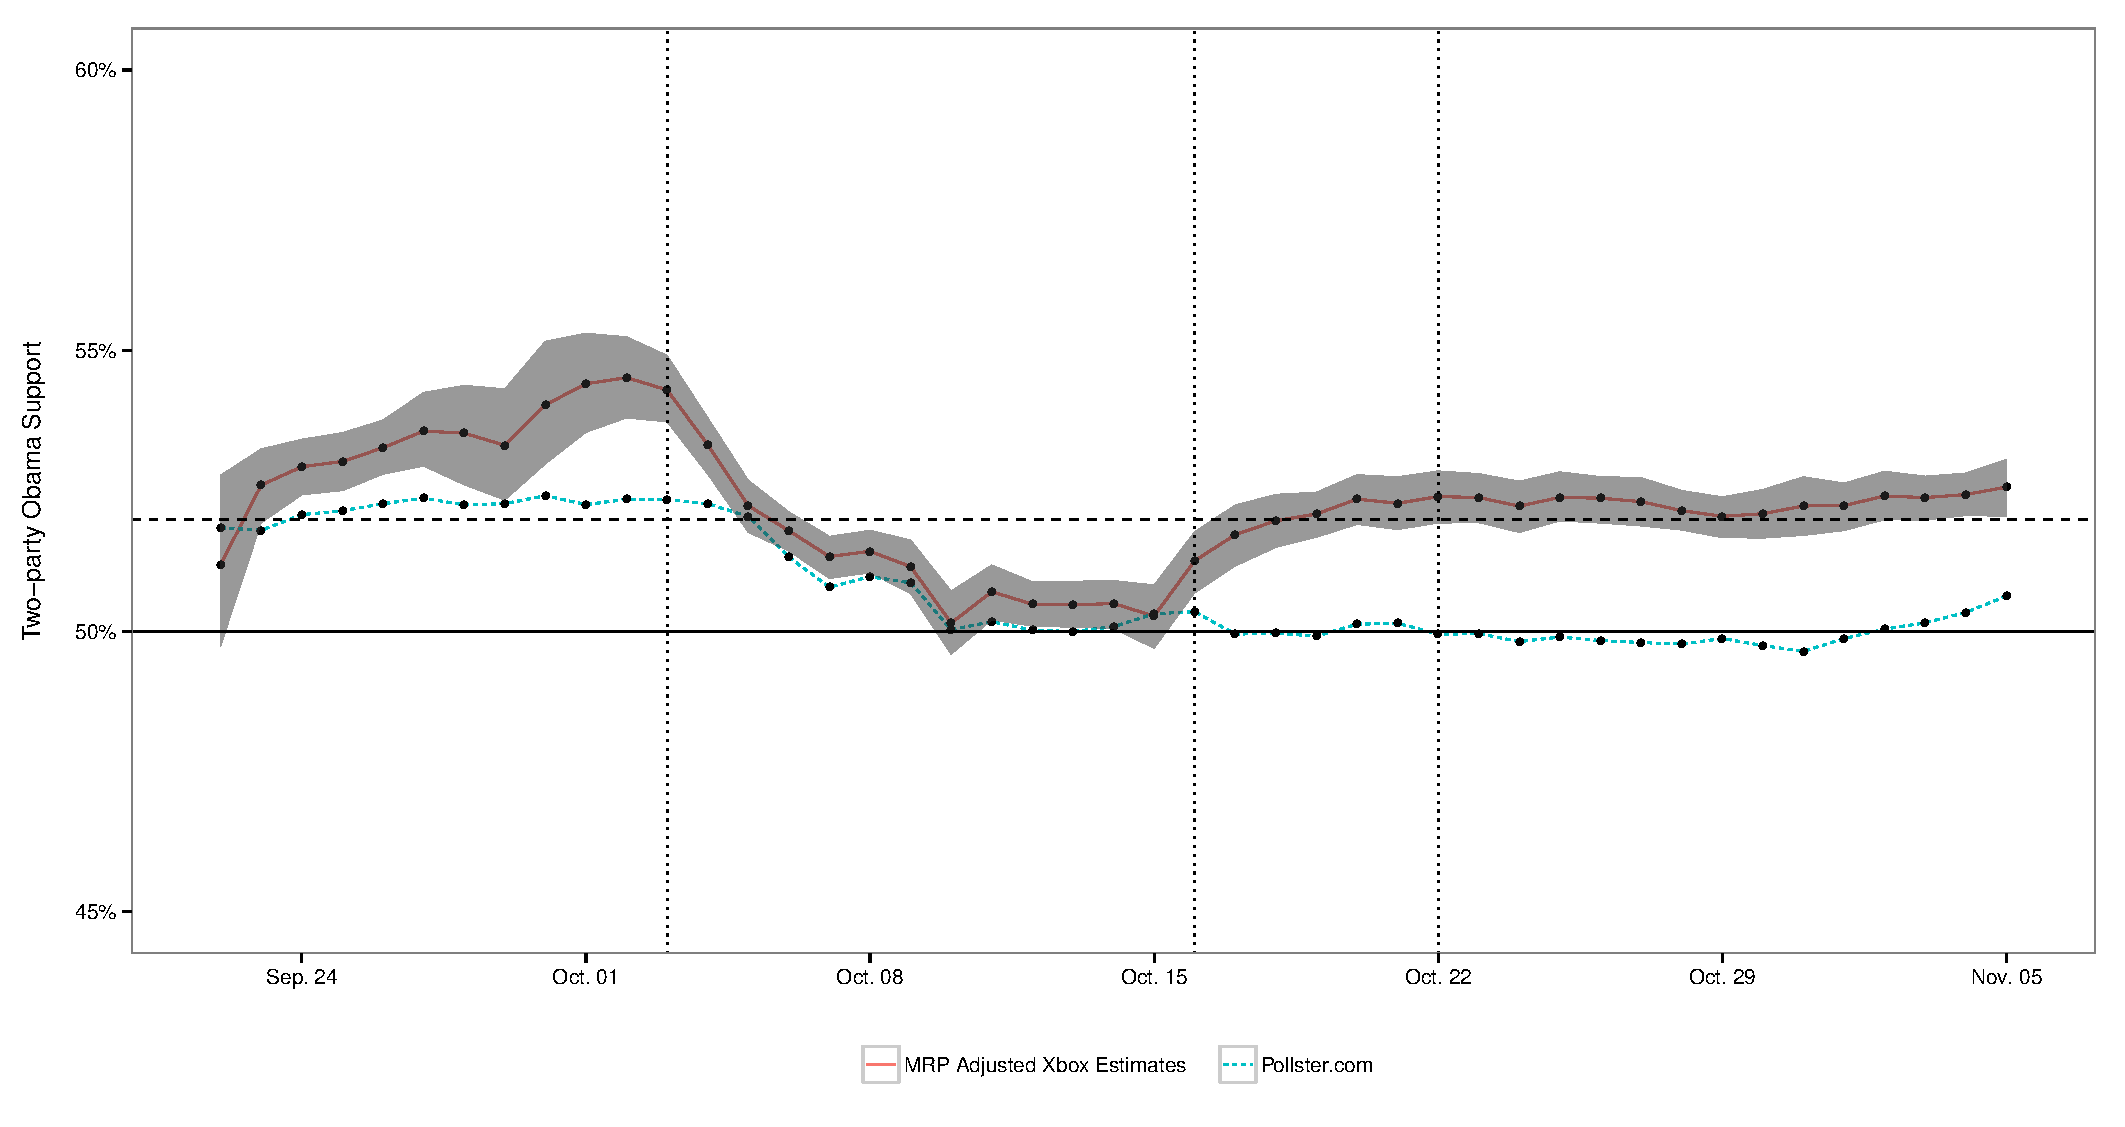
\includegraphics[width=.8\textwidth]{mrp_snapshots_national}
    \end{figure}
  \end{itemize}
\end{frame}

\begin{frame}
  \frametitle{State-level Results of MRP adjustments}
  \begin{itemize}
    \item Furthermore, due to the flexibility of MRP, we can break down the daily
      snapshots by states. The results from 12 largest states are plotted below
      \begin{figure}[htbp]
        \centering
        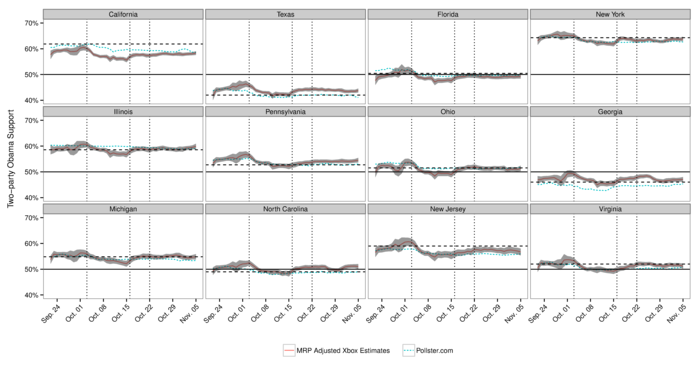
\includegraphics[width=.9\textwidth]{mrp_snapshots_state}
      \end{figure}
  \end{itemize}
\end{frame}

\begin{frame}
  \frametitle{Demographic Subgroups Results of MRP adjustments}
  \begin{itemize}
  \item Comparison between the 2012 exit poll estimates and MRP last day
    snapshots for demographic subgroups and two-way interacted demographic
    subgroups are also shown
    \begin{figure}[htbp]
      \centering
      \includegraphics[width=.8\textwidth]{"demo_group_marginals"}
      \caption{Demographic subgroups two-party Obama support.}
    \end{figure}
  \end{itemize}
\end{frame}

\begin{frame}
  \frametitle{Demographic Subgroups Results Cont'd}
  \begin{figure}[htbp]
    \centering
    \includegraphics[width=.6\textwidth]{"demo_groups_two_way_interaction"}
    \caption{Two-way interaction demographic subgroups two-party Obama support.}
  \end{figure}
\end{frame}

\begin{frame}
  \frametitle{From Daily Snapshots to Election Day Prediction}
  \begin{itemize}
  \item One final step is required to convert the daily snapshots to election day
    prediction.
  \item We follow the approach of Erikson and Wlezien (2008). A regression is fit
    on historical top-line data and actual election outcomes (from 2000, 2004 and
    2008 elections) and projection is made with the MRP adjusted snapshots for
    2012.
  \end{itemize}
\end{frame}


\begin{frame}
  \frametitle{Results of Prediction}
  \begin{itemize}
  \item The daily predictions of the 12 largest states are plotted below
    \begin{figure}[htbp]
      \centering
      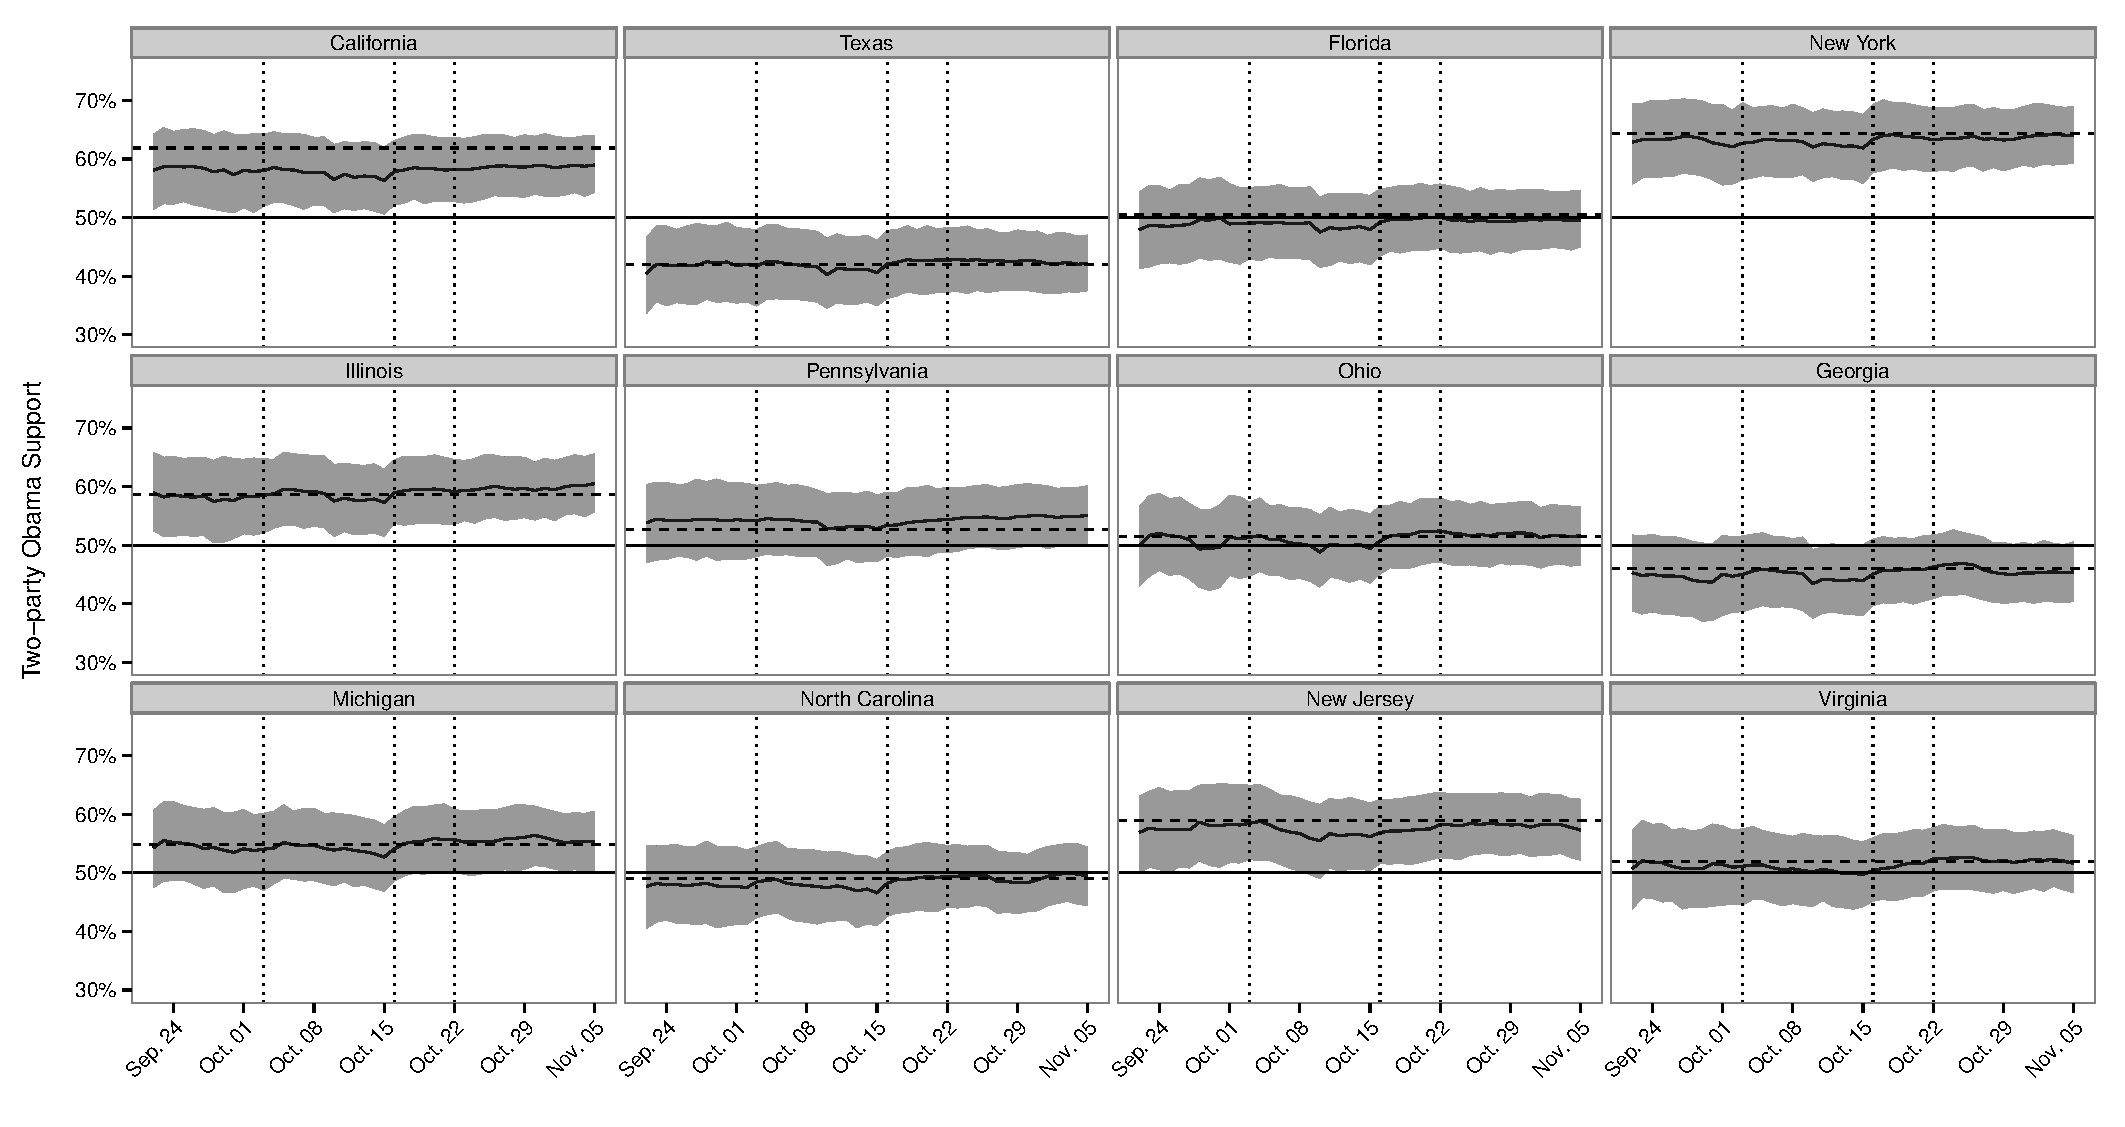
\includegraphics[width=.8\textwidth]{projected_voteshare_state}
    \end{figure}
  \end{itemize}
\end{frame}

\begin{frame}
  \frametitle{Results of Prediction Cont'd}
  \begin{itemize}
  \item Comparison with Prediction Market Data
    \begin{figure}[htbp]
      \centering
      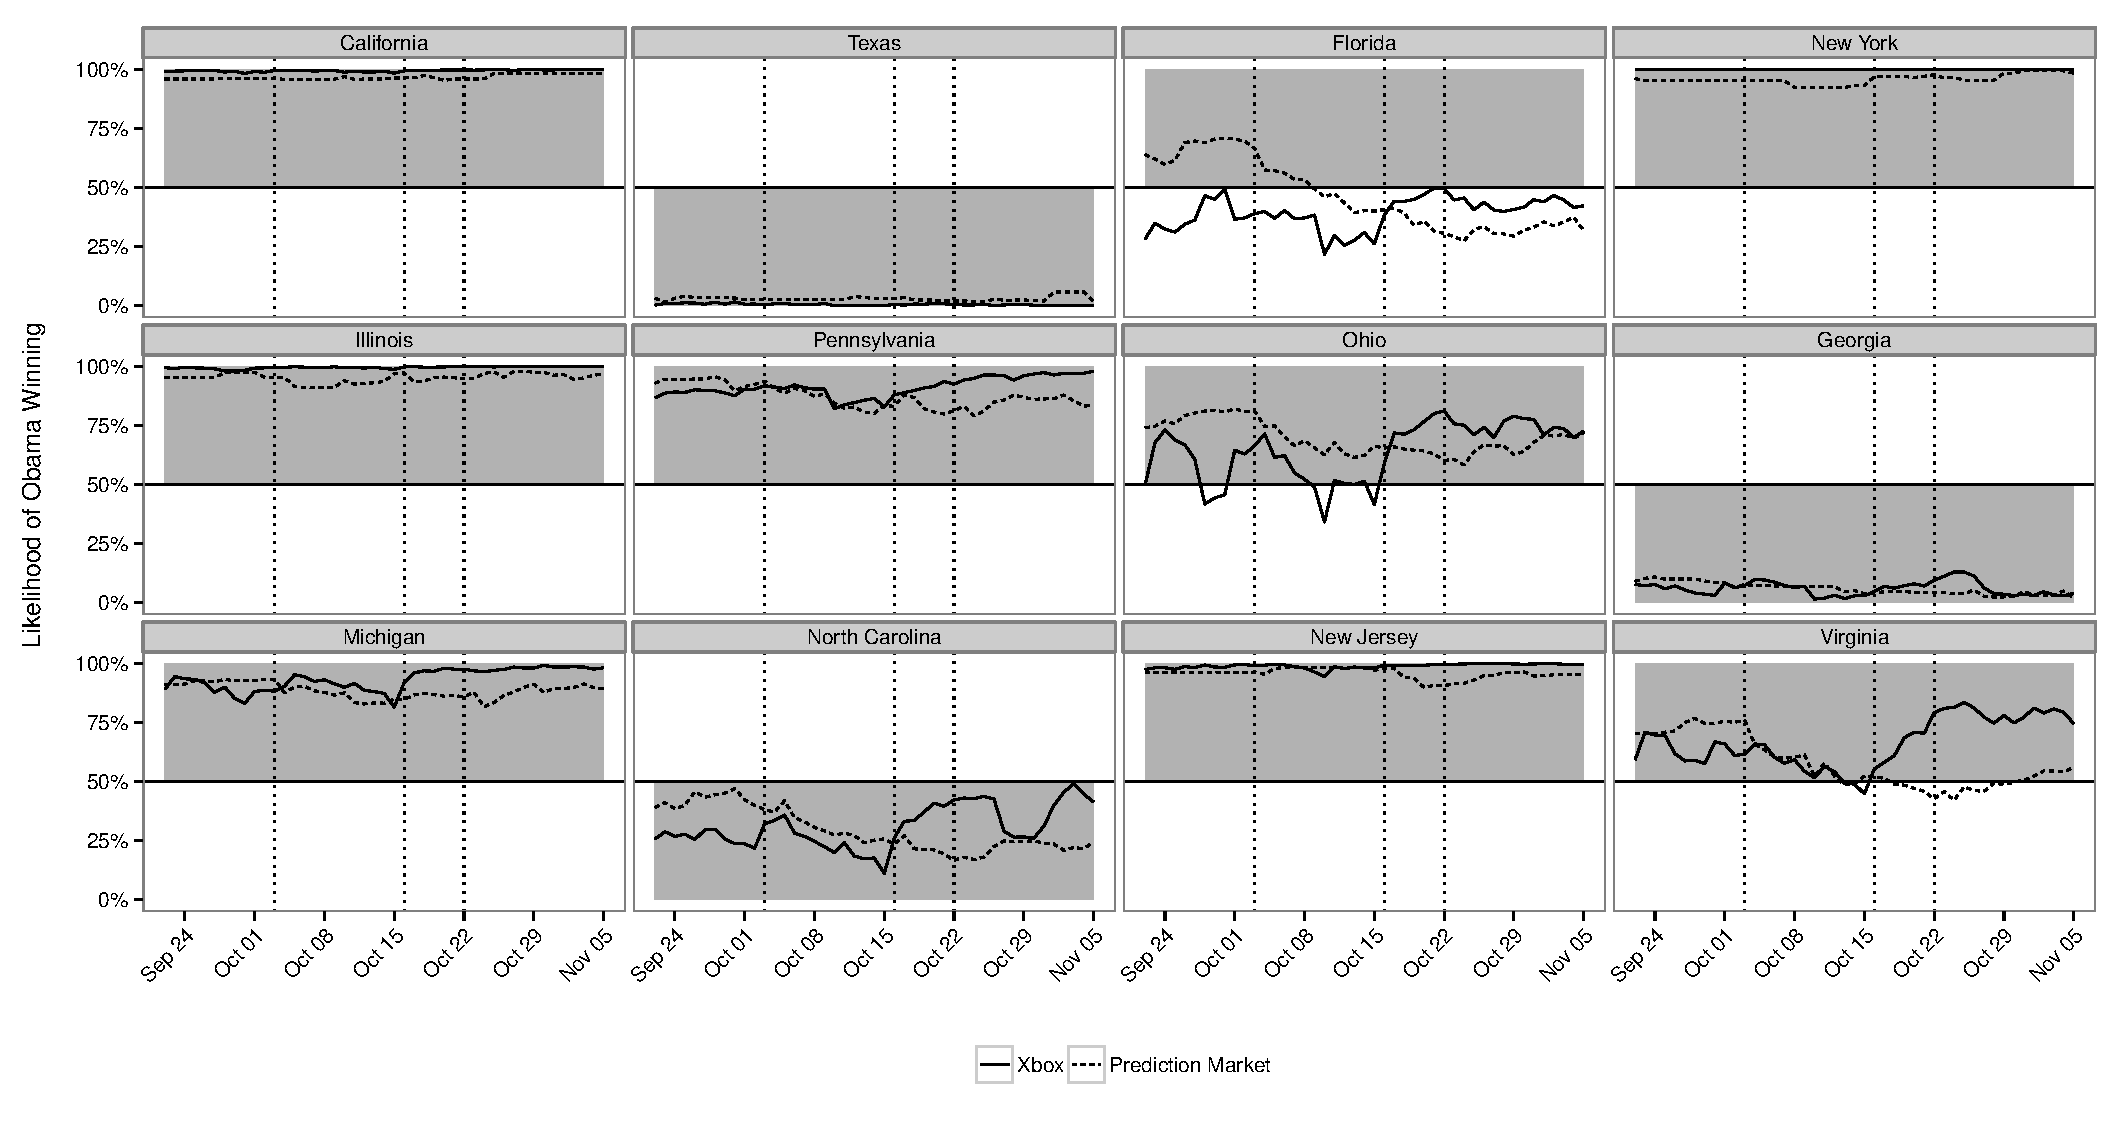
\includegraphics[width=.8\textwidth]{pred_market_xbox_comp}
    \end{figure}
  \end{itemize}
\end{frame}

\begin{frame}
  \frametitle{Results of Prediction Cont'd}
  \begin{itemize}
  \item The daily predictions of Obama's electoral votes.
    \begin{figure}[htbp]
      \centering
      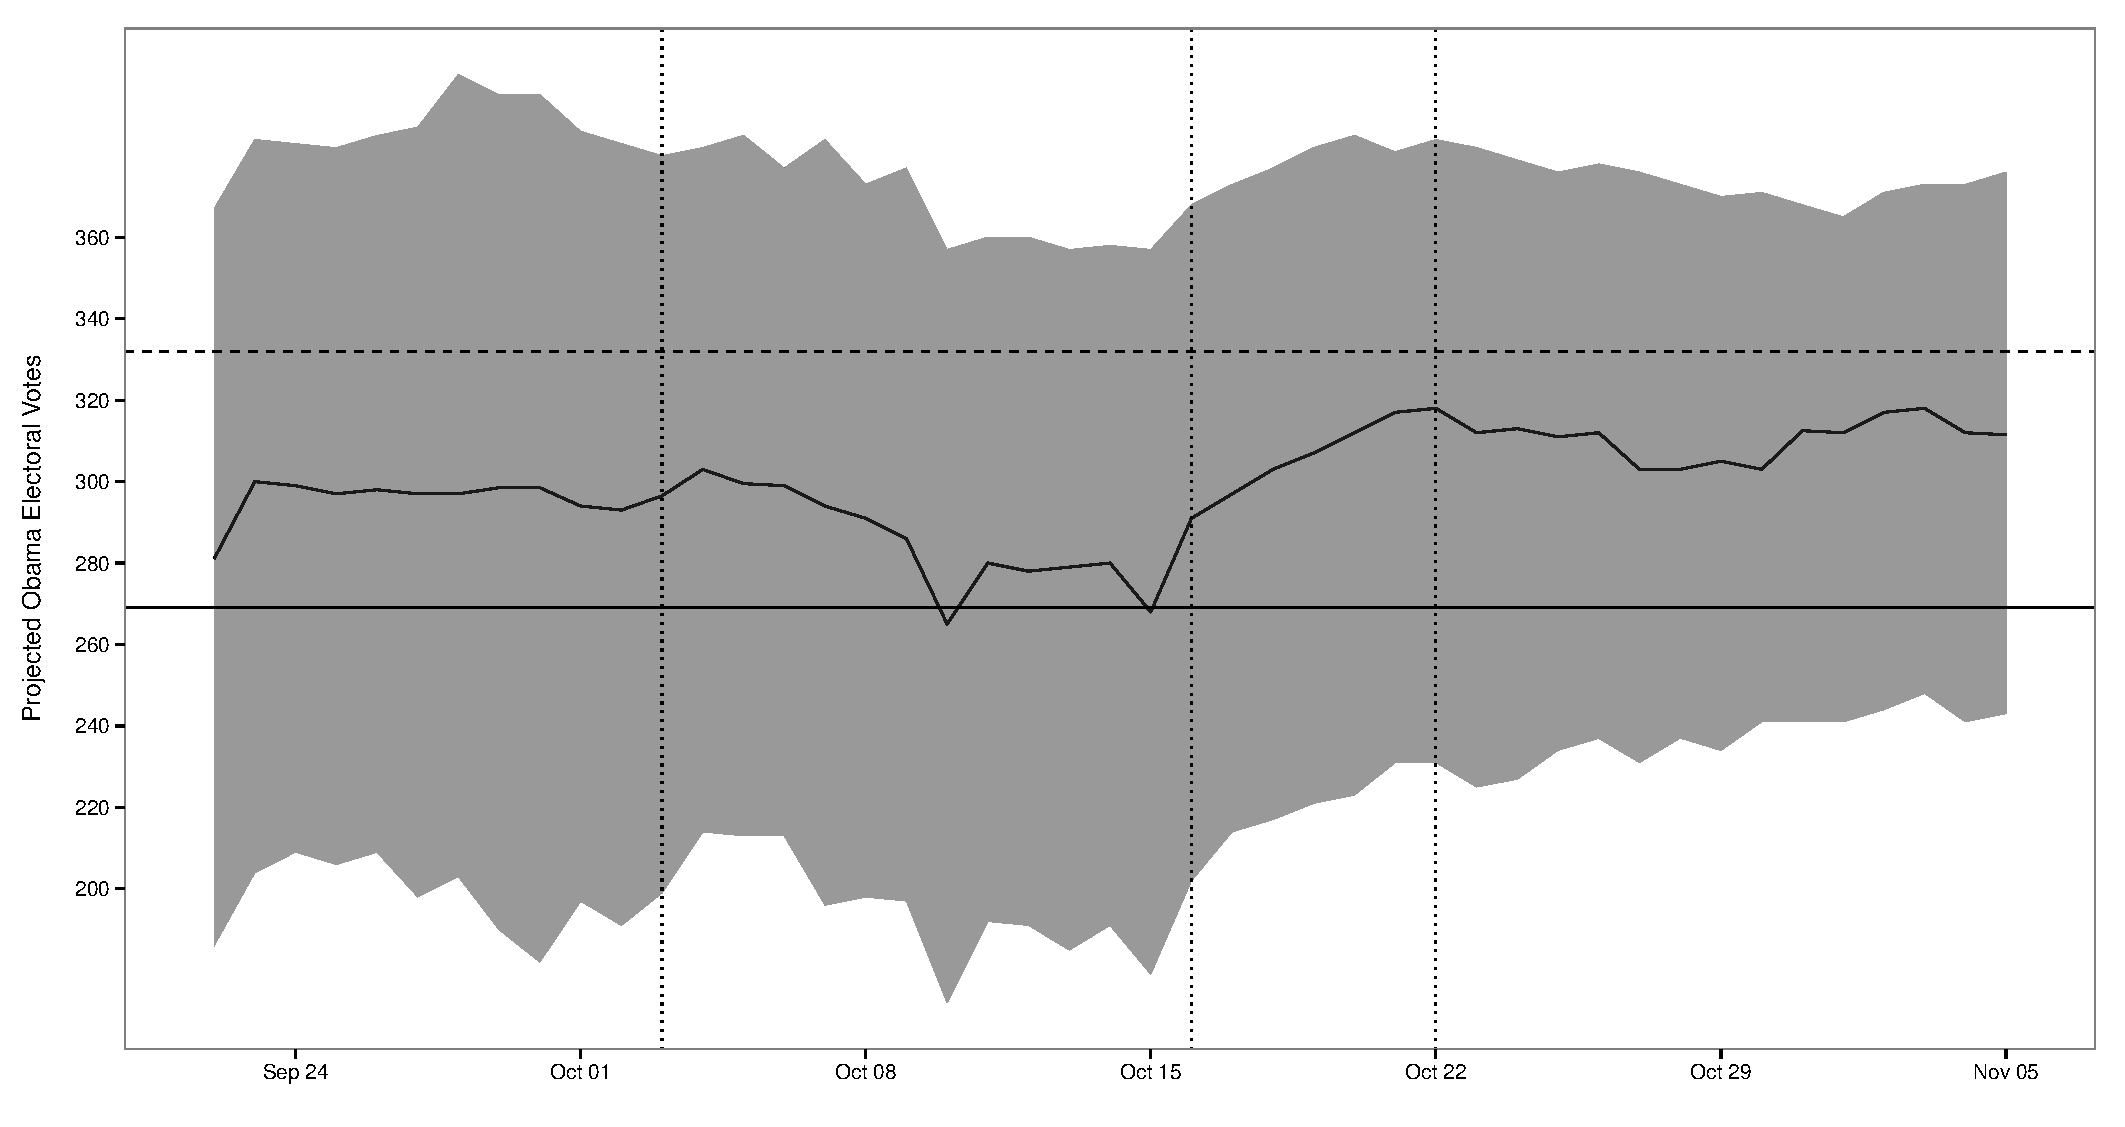
\includegraphics[width=.8\textwidth]{electoral_vote_dist_over_time}
    \end{figure}
  \end{itemize}
\end{frame}

\begin{frame}
  \frametitle{Future Work}
  \begin{itemize}
  \item Apart from the prediction of final election outcomes, there are other
    interesting questions concerning the presidential campaign, such as
    convention bounce.
  \item Based on MRP adjusted daily snapshots, we can quantify the proportion of
    convention bounce due to actual voting intent shift and the proportion due to
    partisan response rate shift resulting from voters' enthusiasm.
  \item Historical data could be traced in public opinion database to study the
    historical changes.
  \end{itemize}
\end{frame}

\begin{frame}
  \frametitle{References}
  \begin{itemize}
  \item Wang, Wei and Rothschild, David and Goel, Sharad and Gelman, Andrew,
    2013. Forecasting Elections with Nonrepresentative Polls. Technical Report.
  \item Erikson, Robert S and Wlezien, Christopher, 2008. Are political markets
    really superior to polls as election predictors? Public Opinion Quarterly.
  \end{itemize}
\end{frame}

\section[Cross-validation]{Use of Cross-validation in Comparing Hierarchical Models}
\begin{frame}
  \frametitle{Introduction}
  \begin{itemize}
  \item Multilevel models are effective tools in survey research.
  \item Cross-validation is a very popular method for estimating generalization
    errors and controlling for overfitting.
    \pause
  \item We want to compare the performance of multilevel models and traditional
    models using cross-validatory metrics.
  \end{itemize}
\end{frame}

\subsection{Model Comparison in A Decision Theoretic Framework}
\begin{frame}
  \frametitle{A Formal Model Comparison Framework}
  \begin{itemize}
  \item Our focus is on predictive power/generalization error.
  \item To take a decision theoretic view, the predictive loss incurred by a
    decision action $\alpha$ based on a model $M$ in face of future observation
    $\tilde y$ under loss function $l$ is given below
    \begin{equation*}
      PL(p^t, M, D)=E_{p^t}l(\tilde y, a_M)=\int l(\tilde y, a_M) p^t(\tilde y)d\tilde y,
    \end{equation*}
  \item We use the whole predictive distribution $p(\tilde y|D,M)$ as the
    decision action $\alpha$ and log loss, the predictive loss materializes as
    \begin{equation*}
      PL(p^t, M, D)=E_{p^t}\log p(\tilde y|D, M)=-\int p^t(\tilde y) \log p(\tilde y|D, M) d\tilde y
    \end{equation*}
  \end{itemize}
\end{frame}

\begin{frame}
  \frametitle{Predictive Errors and Empirical Counterparts}
  \begin{itemize}
  \item We can subtract the entropy of the true distribution $p^t(\tilde y)$
    from the predictive loss to obtain the predictive error
    \begin{align*}
      PE(p^t, M, D)&= PL(p^t, M, D) - LB(p^t) \\  
      &=-\int p^t(\tilde y) \log p(\tilde y|D, M) d\tilde y+\int p^t(\tilde y) \log p^t(\tilde y) d\tilde y.
    \end{align*}
  \item The scale of the predictive error is more interpretable.
  \item We need to estimate the two parts in the predictive error.
  \end{itemize}
\end{frame}

\begin{frame}
  \frametitle{$k-$fold Cross-validation for Predictive Loss}
  \begin{itemize}
  \item $k-$fold cross-validation estimate of the predictive loss is given by
    \begin{align*}
      \widehat{PL}^{\text{CV}}(M, D) &=-\,\frac{1}{N}\sum_{k=1}^K\sum_{i\in
        \text{test}_k}\log p(y_i|D^k, M)\\
      &=-\,\frac{1}{N}\sum_{i=1}^N\log p(y_i|D^{(\backslash i)}, M),
\end{align*}
where $D^k$ represents the $k$\textsuperscript{th} training set and
$D^{(\backslash i)}$ denotes the training set that excludes the
$i$\textsuperscript{th} observation.
  \end{itemize}
\end{frame}

\begin{frame}
  \frametitle{Lower Bound and Data Partition}
  \begin{itemize}
  \item The lower bound of the predictive loss, i.e., the entropy of the true
    distribution, is approximated by the in-sample training loss the of saturated
    model $M_s$, which gives an estimates of the predictive error
    \begin{align*}
      \widehat{PE}(M, D)&=\widehat{PL}^{\text{CV}}(M,D)-TL(M_{\text{s}},D)\\  \label{eq:esti_preerror}
      &= -\,\frac{1}{N}\sum_{i=1}^N\log p(y_i|D^{(\backslash i)},
      M)+\frac{1}{N}\sum_{y\in D}\log p(y | D, M_{\text{s}}).
    \end{align*}
  \item Partition of structured data in cross-validation could be tricky. One
    possibility is to do cluster sampling, in which we fit the model on training
    cells and test on hold-out cells. We adopt a stratified sampling approach and
    partition each cell into training and testing sets.
  \end{itemize}
\end{frame}
\subsection{Data and Model Descriptions}
\begin{frame}
  \frametitle{CCES 2006 Survey Data}
  \begin{itemize}
  \item Collaborative Congressional Election Survey 2006 is a national stratified
    sample of size 30,000, with a wide variety of response outcomes. 
  \item We convert all outcomes (71 in total) into binary, and fit multilevel
    models for each of the outcomes.
  \item This provides an ideal setting to evaluate cross-validation.
  \end{itemize}
\end{frame}

\begin{frame}
  \frametitle{Model Descriptions}
  \begin{itemize}
  \item For simplicity, we only consider two predictors, state and income. The
    data is cross-tabulated by these two variables, and for respondents in cell
    $(j_1,j_2)$, the probability that they give a positive response is
    $\pi_{j_1,j_2}$, which is modeled with a logistic regression
    $\text{logit}(\pi_{j_1j_2})=\bm Z\bm\beta$, in which $\bm Z$ is the design
    matrix and $\bm\beta$ includes the main and interaction effects.
  \item We compare three models
    \begin{itemize}
    \item Complete pooling:
      $    \pi_{j_1j_2}=\text{logit}^{-1}\left(\beta^{\text{state}}_{j_1}+\beta^{\text{inc}}_{j_2}\right)$
    \item No pooling (saturated model): $
      \pi_{j_1j_2}=\text{logit}^{-1}\left(\beta^{\text{state}}_{j_1}+\beta^{\text{inc}}_{j_2}+\beta^{\text{state*inc}}_{j_1j_2}\right)$
    \item
      Partial pooling:
      $ \pi_{j_1j_2}=\text{logit}^{-1}\left(\beta^{\text{state}}_{j_1}+\beta^{\text{inc}}_{j_2}+\beta^{\text{state*inc}}_{j_1j_2}\right)$, with
      $\beta^{\text{state*inc}}_{j_1j_2}\stackrel{i.i.d.}{\sim} \Phi(\cdot)$.
    \end{itemize}
  \end{itemize}
\end{frame}
\subsection{Results}
\begin{frame}
  \frametitle{The Real Data}
  \begin{itemize}
  \item The estimated predictive errors for all 71 outcomes are plotted
    below. The x-axis is ordered by the training loss of the saturated model. The
    no pooling model gives a bad fit.  Partial pooling does best but in most
    cases is almost indistinguishable from complete pooling under the
    cross-validation criterion.
    \begin{figure}[htbp]
      \centering
      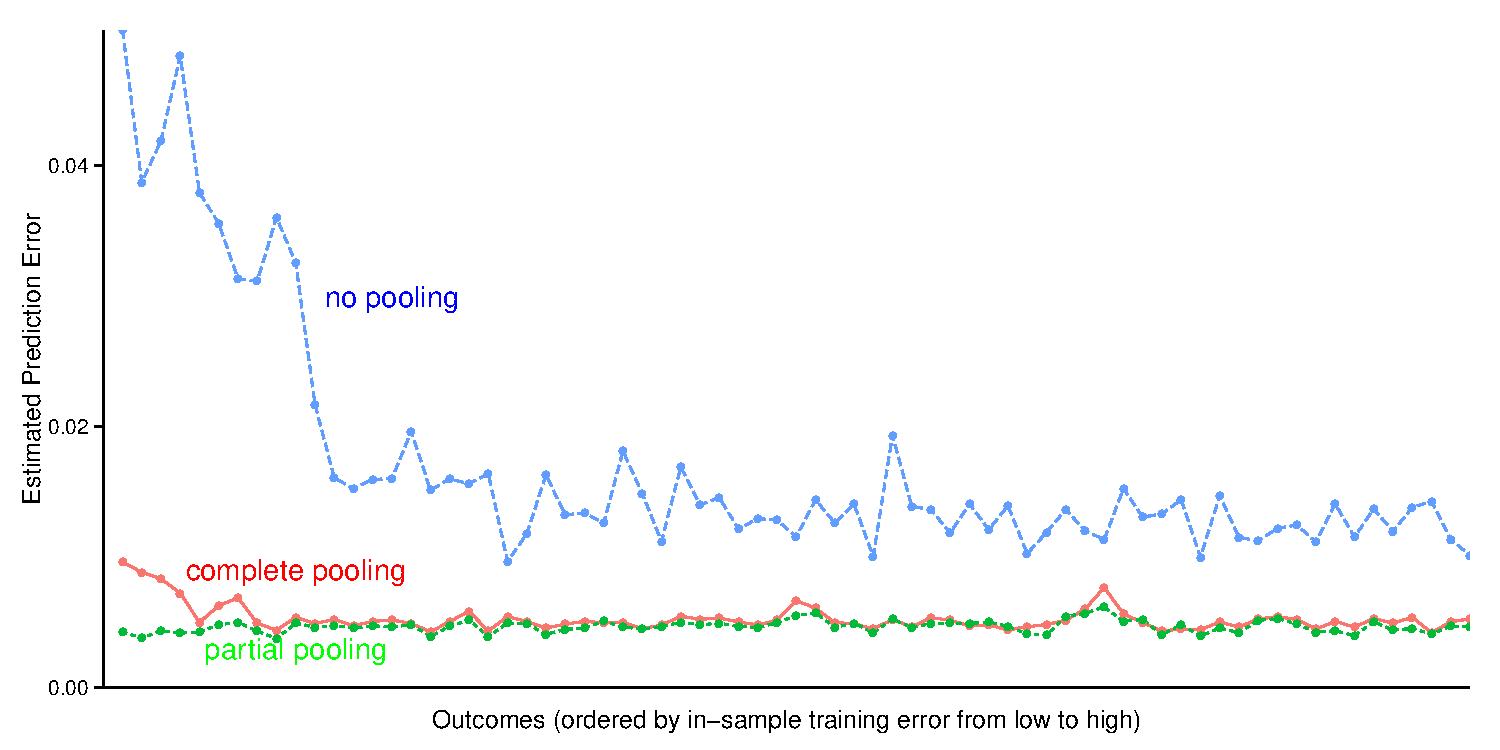
\includegraphics[width=.8\textwidth]{alloutcomesx1.pdf}
    \end{figure}
  \end{itemize}
\end{frame}

\begin{frame}
  \frametitle{Simulated Data: Changing Sample Size}
  \begin{itemize}
  \item From the previous graph, it seems that the multilevel model fails to pick
    up the interaction between income and state. We augment the data set by
    replicating each observation multiple times. 
    \begin{figure}[htbp]
      \centering
      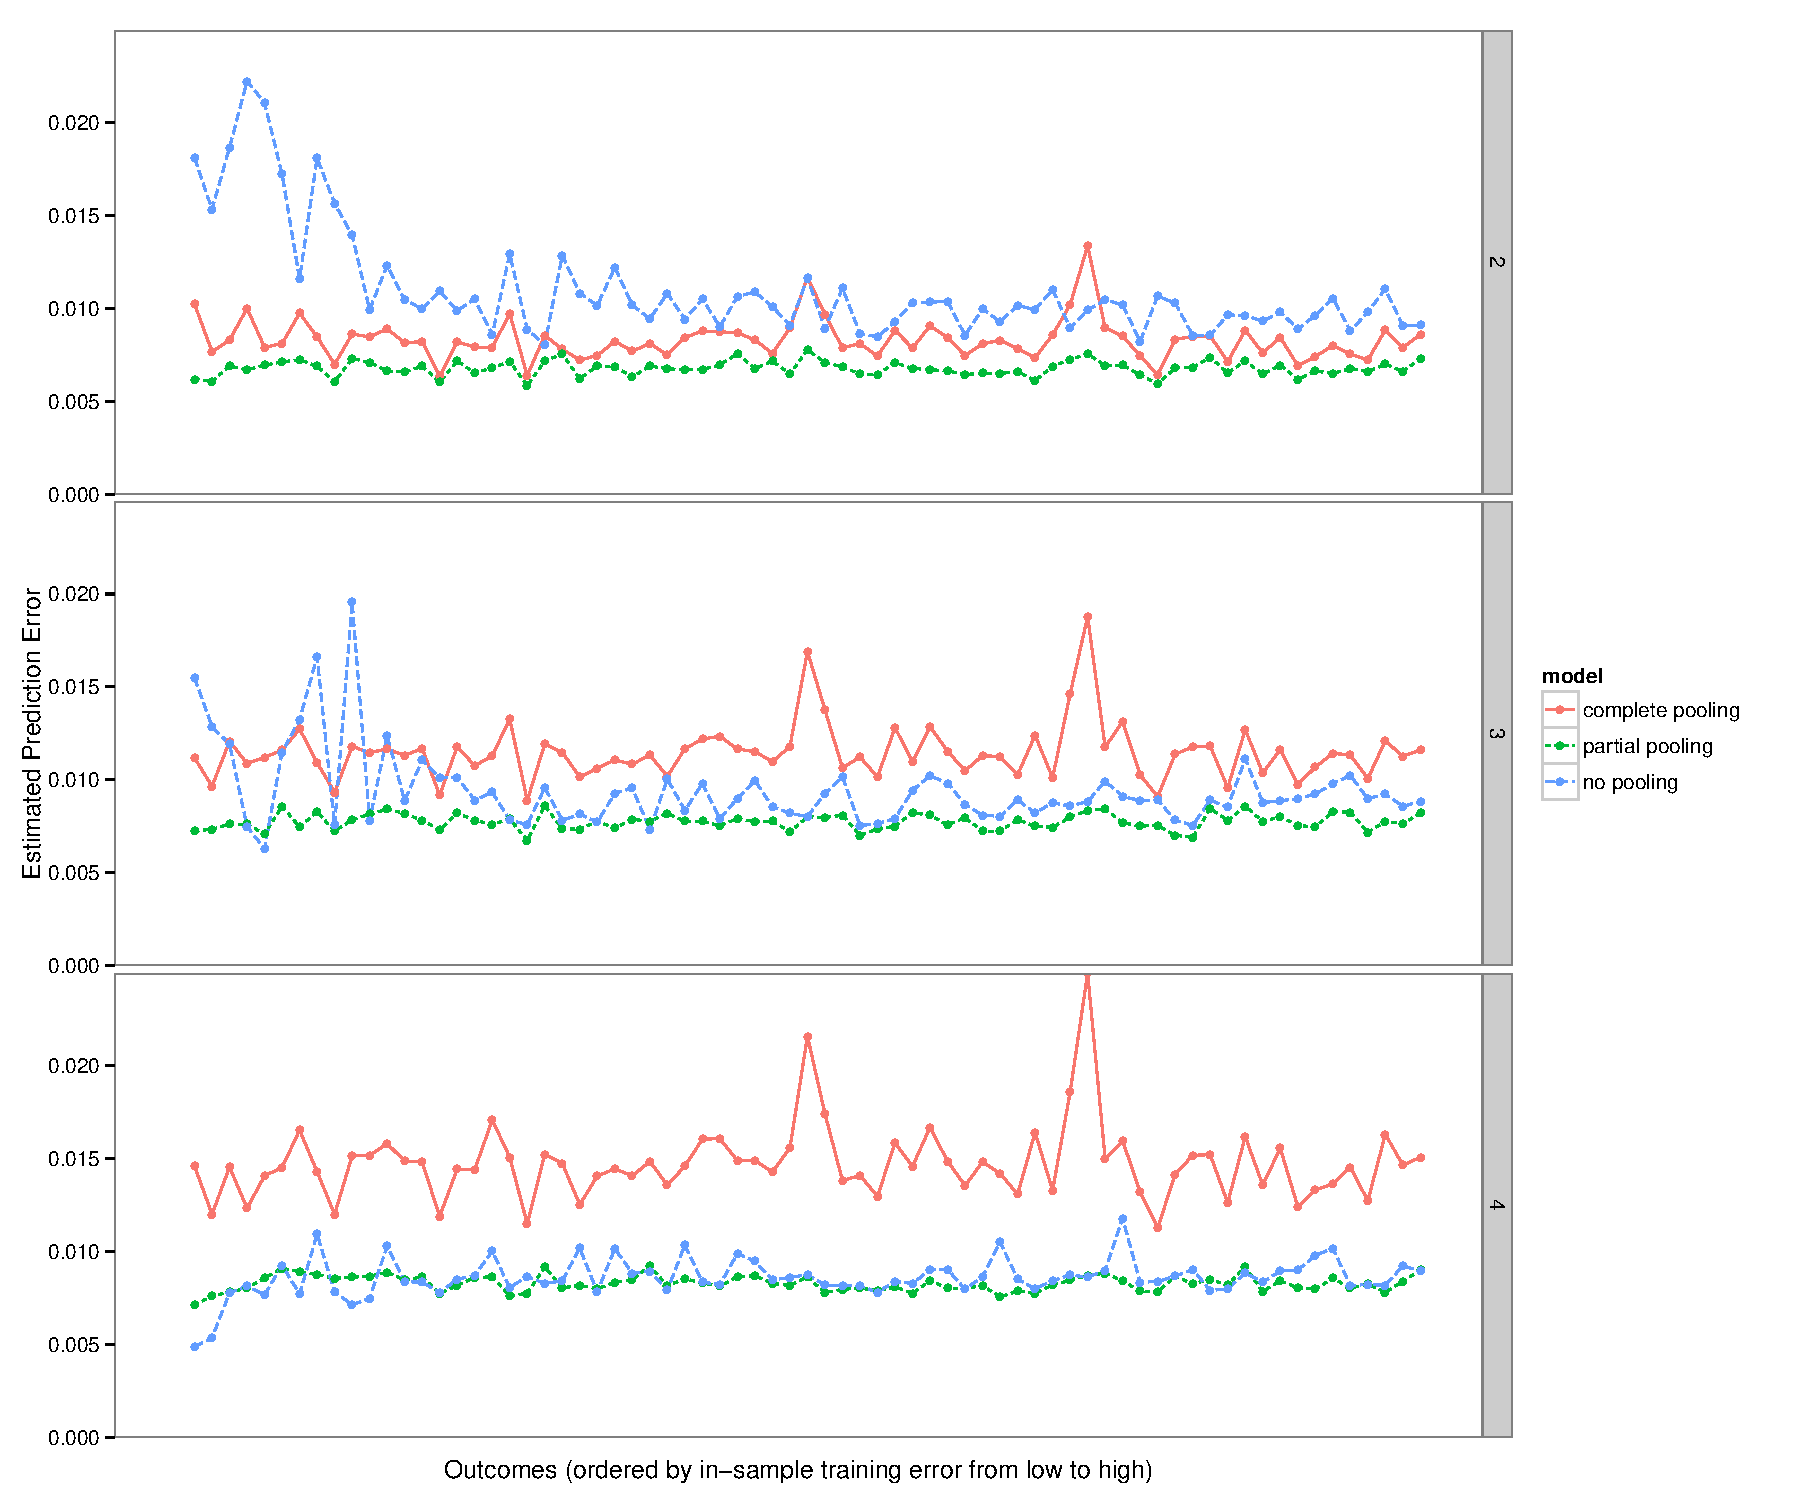
\includegraphics[width=.6\textwidth]{outcome234.pdf}
    \end{figure}
  \end{itemize}
\end{frame}

\begin{frame}
  \frametitle{Simulated Data: Changing Sample Size Cont'd}
  \begin{itemize}
  \item We also look at one particular outcome, two-party republican support in
    the congressional election. Again, partial pooling performs the best, but its
    performance is roughly matched by no pooling in large sample sizes and by
    complete pooling in small sample sizes.
    \begin{figure}[htbp]
      \centering
      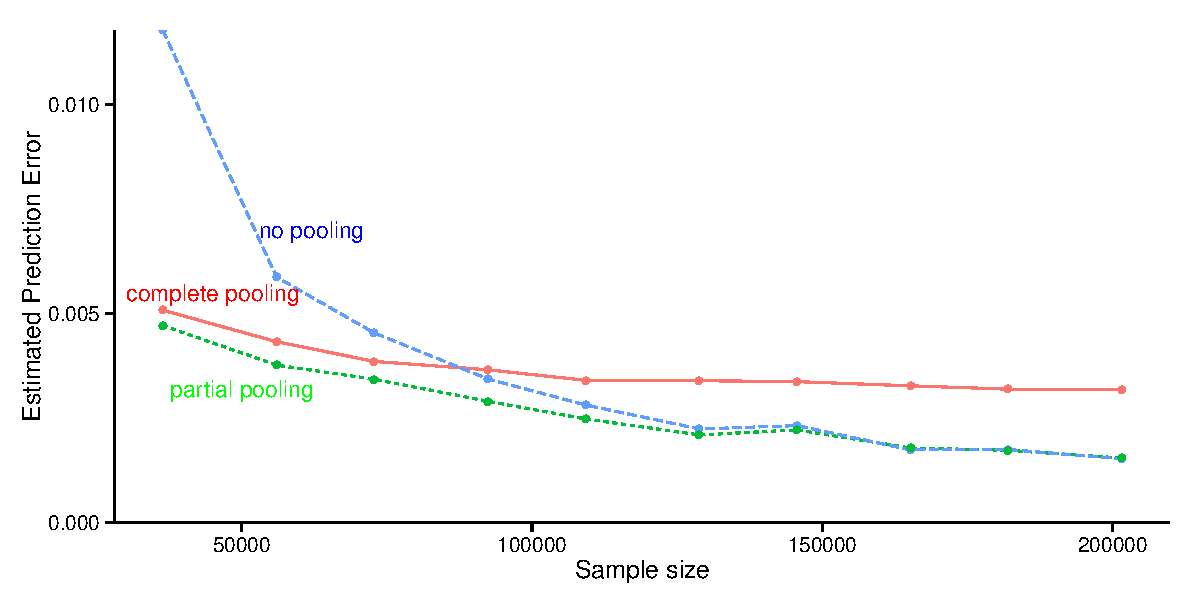
\includegraphics[width=.8\textwidth]{hourvote.pdf}
    \end{figure}
  \end{itemize}
\end{frame}

\begin{frame}
  \frametitle{Simulated Data: Balancedness of Cells}
  \begin{itemize}
  \item Another factor underlying the relative performance of different models
    might be the highly-unbalanced structure of the survey data. We simulate data
    of the same sample size and cell proportion as the original data but with
    balanced cell sample sizes.
    \begin{figure}[htbp]
      \centering
      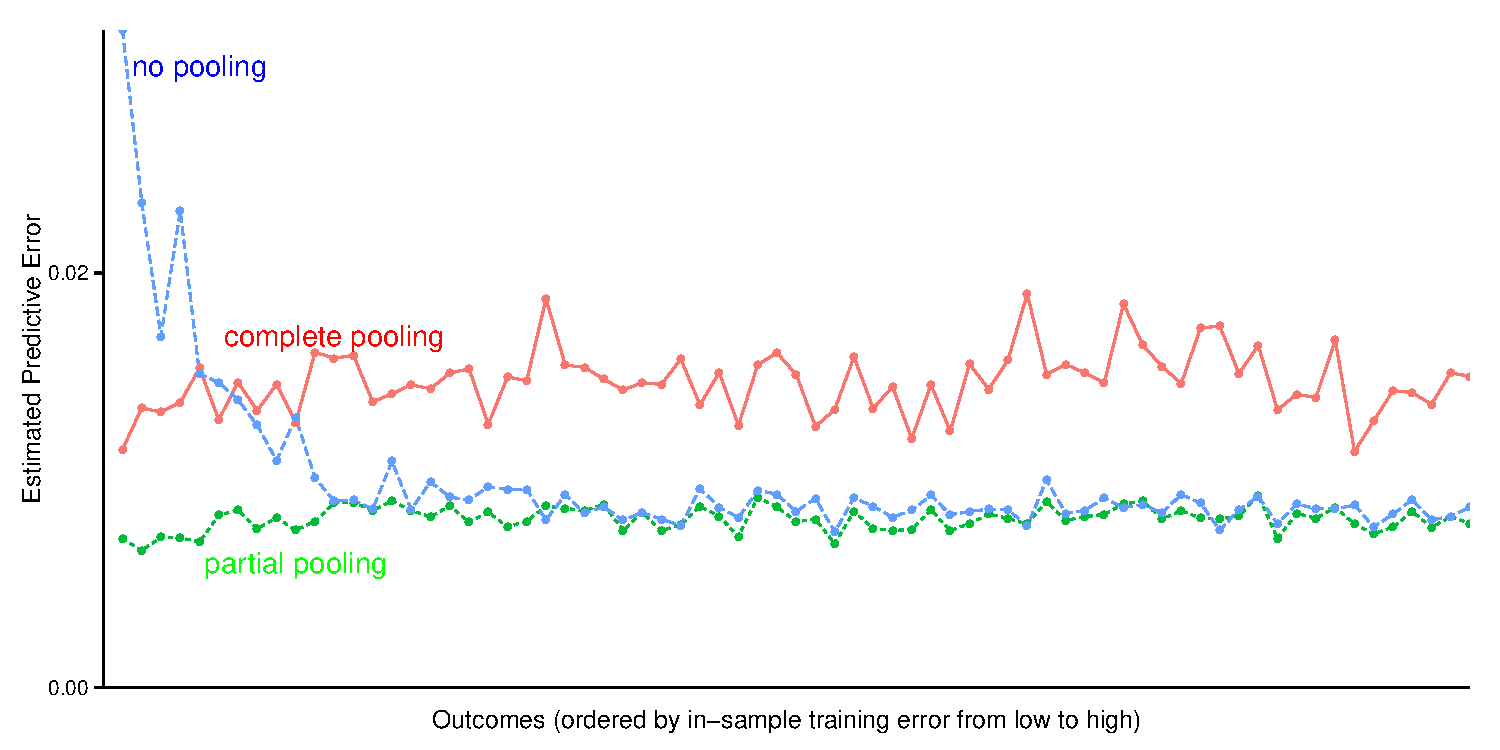
\includegraphics[width=.8\textwidth]{alloutcomesxbal.pdf}
    \end{figure}
  \end{itemize}
\end{frame}

\begin{frame}
  \frametitle{Simulated Data: Balancedness of Cells Cont'd}
  \begin{itemize}
  \item In this case, we also let sample size grow and see the relative
    performance of the three models for the congressional election republican
    vote.
    \begin{figure}[htbp]
      \centering
      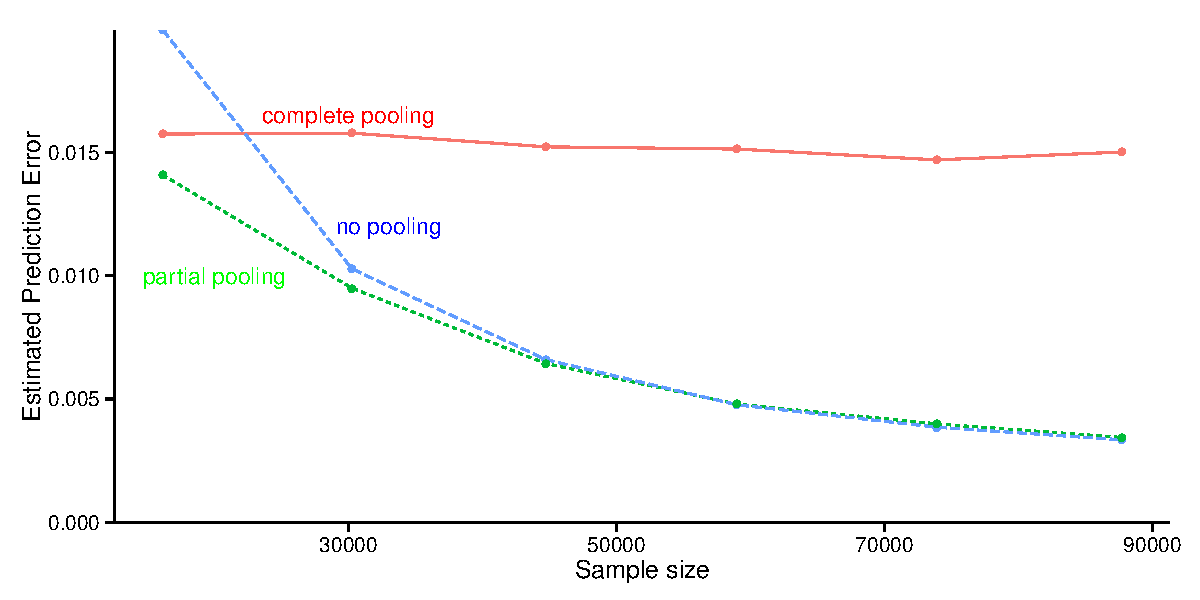
\includegraphics[width=.8\textwidth]{hourvote_bal.pdf}
    \end{figure}
  \end{itemize}
\end{frame}

\begin{frame}
  \frametitle{Discussion}
  \begin{itemize}
  \item Multilevel models capture the important interactions that are not included
    in the complete pooling model, while at the same time avoiding the inevitable
    overfitting from the no pooling model.  
  \item However, the improvement of the multilevel model as given by
    cross-validation is surprisingly tiny, almost negligible to unsuspecting
    eyes.
  \item Simulations based on real data show that sample size and structure of the
    cross-tabulated cells play important roles in the relative margins of
    different models in cross-validation based model selection.
  \item Caution should be exercised in applying cross-validation for model
    selection with structured data.
  \end{itemize}  
\end{frame}

\begin{frame}
  \frametitle{References}
  \begin{itemize}
  \item Wang, Wei and Gelman, Andrew, 2013. A problem with the use of
    cross-validation for selecting among multilevel models. Technical Report.  
  \item Vehtari, Aki and Ojanen, Janne, 2013. A survey of Bayesian predictive
    methods for model assessment, selection and comparison. Statistics Survey.
  \end{itemize}
\end{frame}

\end{document}
